\documentclass{proseminar}

\begin{document}

\conferenceinfo{Albert-Ludwigs Universit\"at Freiburg\\Technische Fakult\"at, Institut f\"ur Informatik\\Lehrstuhl f\"ur Datenbanken \& Informationssysteme}{}

\title{Trust and Privacy in Social Media \\
\huge Content oriented trust}

\numberofauthors{1} 
\author{
Tim Schmiedl\\
\email{tim.schmiedl@neptun.uni-freiburg.de}
}

\maketitle

\section{Introduction}
* Microblogging is a well-established paradigm for interaction in online social networks. 

* real-time fashion 

* mobile internet devices 

* propagating news and information about developing events 

% =========================

\subsection*{Current Situation \& Potential}
+ new ranking strategy that considers popularity of tweets

* Besides helping to communicate relevant events on a day-to-day basis, microblogging can be particularly helpful during emergency and/or crisis
situations 

* provide real-time information from the actual location where the crisis is unfolding. This
information often spreads faster and to a wider audience than what traditional news
media sources can achieve.

% =========================

\subsection*{Problems}
+ This ranking method, however, has not taken into account content relevance or the twitter account.

+ a large amount of pointless tweets may flood the relevant tweets

+ spam is not avoided in rankin method

* variety of content; NEWS / Chat

* valuable to the user and its immediate circle offriends VS  valuable to a broader community

* NO DISTINCTION between news / chat

% =========================

\subsection*{Goals of the Papers}
+ In this paper,  a method to rank the tweets  based on their content relevance to the query

+  learning to rank approach

+  best set of features

* In this work we focus mostly on the credibility of newsworthy information is a correlation between how information propagates and the credibility 

* aid them in the process of discovering reliable information.  achieved in an automatic way using features extracted from information cascades


% =========================
% =========================
% =========================


\section{Twitter Case Study}
* from P1: Predicting information credibility in time-sensitive social media

* earthquake that hit Chile on February 2010

*  Event characterization

*  Twitter reaction: Information propagation behavior \& False rumor propagation


% =========================
% =========================
% =========================

\section{Proposed Method: Ranking of \\Tweets}
+ method of P2: An Empirical Study on Learning to Rank of Tweets

+ Learning to Rank: data-driven approach

+ RankSVM for training the ranking model

\begin{figure}[h]
\centering
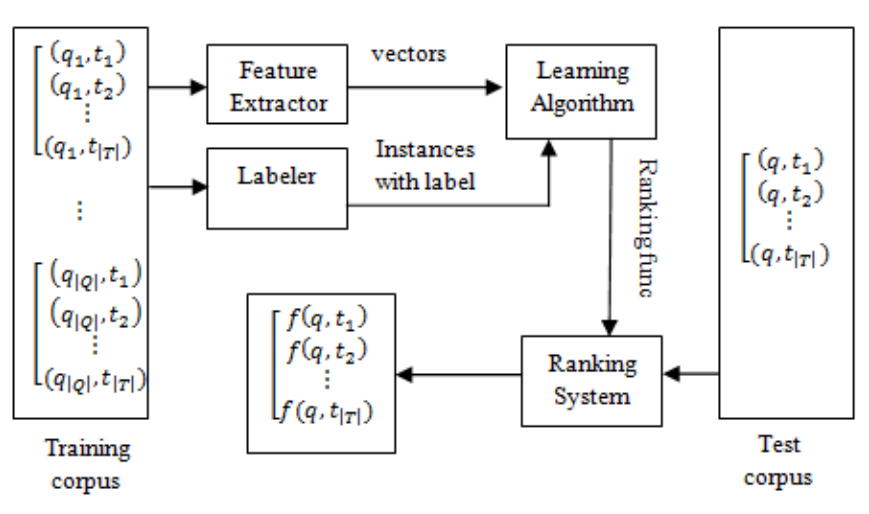
\epsfig{file=img/p2_overview.png, width=0.45\textwidth}
\caption{General Paradigm of Learning for Tweets Ranking}
\end{figure}

+ Features for Ranking: Content relevance features, Twitter specific features, Account authority features

\subsubsection*{Content relevance features}

+ three differen content relevance features

+ Okapi BM25: content relevance between query and tweet

+ Similarity  of  contents: cosine sim for pair of tweets

+ Length: number of words

\subsubsection*{Twitter Specific Features}
+ URL \& URL count

+ Retweet Count

+ Hash Tag Score

+ Reply

+ OOV (Words out of vocabulary)

\subsubsection*{Account Authority Features}
+ There are three important relations between users in Twitter: follow, retweet, and mention. 

+ user are more authoritative: more followers, been mentioned in more tweets, listed in more lists and retweeted by more important users

+ tweet is more likly to be informative if posted or retweeted by authoritative user

+ Scores: Follower, Mention, List, Popularity (computed by PageRank)

% =========================
% =========================
% =========================

\section{Proposed Method: Prediction\\ Model for Tweets}
* method of P1: Predicting information credibility in time-sensitive social media

* The main focus credibility of time-sensitive information, in particular on current news events. 

* newsworthiness of a discussion topic, and that of determining its credibility, are equally important


\subsection{Retrieving and Labeling of Data}
* information cascade, which is composed of all of the messages which usually accompany newsworthy events

* detected by Twitter Monitor (keyword-based query), detection of events see Mathioudakis and Koudas, 2010

* 2 month monitoring, keep topics with at most 10.000 tweets = 2.500 topics w  1,873,000 messages (initial topic data)


\subsubsection*{Newsworthyness}
* first step seperate newsworthy topics vs conversation/chat etc.: manual data labeleling procress, Crowdsourcing with Mechanical Turk

* human editor label Data as: NEWS / Chat / Unsure

* short summary sentence for the topic, reduce the effect of click spammers

* Result:  35.6 (136 cases) UNSURE, 29.5 percent NEWS (113 cases), 34.9 percent CHAT (134 cases).

\subsubsection*{Credibility}
* second round: newsworthy topics should be rated in credibility

* input is the output of the automatic classifier based on the data extracted in the first step

* 747 topics with NEWS label presented to human evaluator for judgement

* 4 different credibility classes: "almost certainly true" (306 cases), "likely to be false" 31.8 percent (237 cases), "almost certainly false" 8.6
percent (65 cases), 18.6 percent (139 cases) uncertain.

\subsection{Prediction Model for Tweets}
* main hypothesis is that the level of newsworthiness and credibility can be estimated automatically.

\subsubsection*{Automatic discovery of newsworthy topics}
* labeled data as training set for different learning schemes. Bayes Net best for the scenario (Random forest comparable results)

* different factors show credible:

* 1. reactions and emotion, opions, negative/positive sentiments 

* 2. certainty, question info or not?

* 3. sources cited, URLs, popular domain

* 4. propagation characteristics, which user, how many follower etc.

* Feature subsets: Text-only, User subset, Topic subset, Propagation subset

* Text: length of tweet, sentiment-based features, URLs, Twitter-specific: hashtags, user mentions (20 features)

* User: aggregated properties of authors like \#friends \#followers (7 features)

* Topic: most frequent URL, most frequent hashtag, most frequent user mention, and most frequent author (4 features)

*  the propagation-based features, fraction of re-tweets, total number of tweets (7 features)

\begin{figure}[h]
\centering
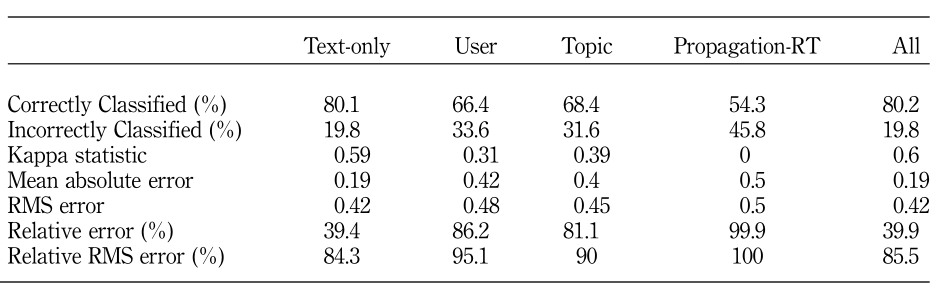
\epsfig{file=img/p1_table_feature_subset.png, width=0.45\textwidth}
\caption{Results for different feature subsets}
\end{figure}

\subsubsection*{Credibility prediction}
* how to automatically assign a credibility level (or score) to a topic deemed newsworthy by our previous classifier

*  binary classification:  CREDIBLE , NOT-CREDIBLE 47.2/52.8 percent. In total, these topics involve 165,312 tweets

*  study how different learning algorithms perform in particular learning scenario

*  predictability of the problem is very difficult, with very moderated k-statistic values (see Evaluation)

* Feature selection:  evaluate 684 subsets, best results with 16 features

* fraction of tweets having a positive/negative sentiment; 

* fraction of tweets with URL, URL top 10.000 urls

* tweets containing:  question mark, exclamation mark, first- /second-person pronoun, emoticons

% =========================
% =========================
% =========================

\section{Evaluation}
\subsection{Predicting information credibility in time-sensitive social media}

\subsubsection*{Credibility}
*  predictability of the problem is very difficult, with very moderated k-statistic values

* main conclusions are that misclassification of not-credible topics as credible is significant, but recall rates are quite acceptable.

* features positive for credibility: more friends, more URLs + urls in popular 10.000, longer in general, negative sentiments

* features negative for credibility: positive polarity, more question and exclamation marks, first and third-persion pronouns

% =========================

\subsection{An Empirical Study on Learning to Rank of Tweets}
\subsubsection*{Dataset}
+ 20 query terms on CrowdEye (5 persons, 5 locations, 5 products and 5 movie names)

+ 159,298 tweets

+ 500 tweets/topic evaluated by human editor: labeled with grade 4 judgements 

+ Excellent  20.9 \% ; Good  10.9\%;  Fair 16.9\%; Bad 51.3\% 

\subsubsection*{Results}
+ different methods tested in Five-fold cross-validation of tweets in 16 queries: chronological order, account  authority,  and  content  relevance + combinded
\begin{figure}[h]
\centering
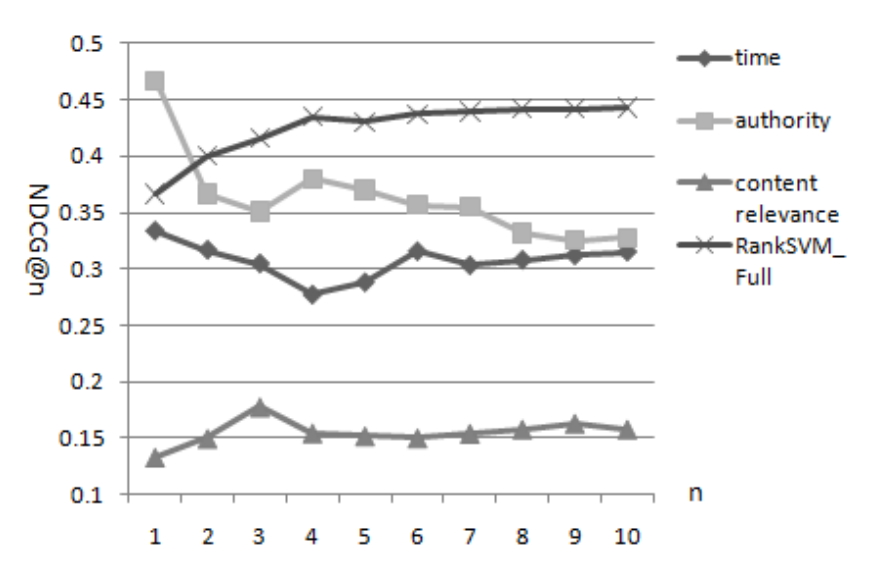
\epsfig{file=img/p2_results.png, width=0.45\textwidth}
\caption{Performance of Four Ranking Methods}
\end{figure}

+ evaluation of the Feature Selection: which are the best features?

+ Combined set of features with best results: URL, Sum\_mention, First\_List, Length, and Important\_follower

+ tested with leave out one, results in figure 3

+ URL is best feature, other features on its own are not significant

\begin{figure}[h]
\centering
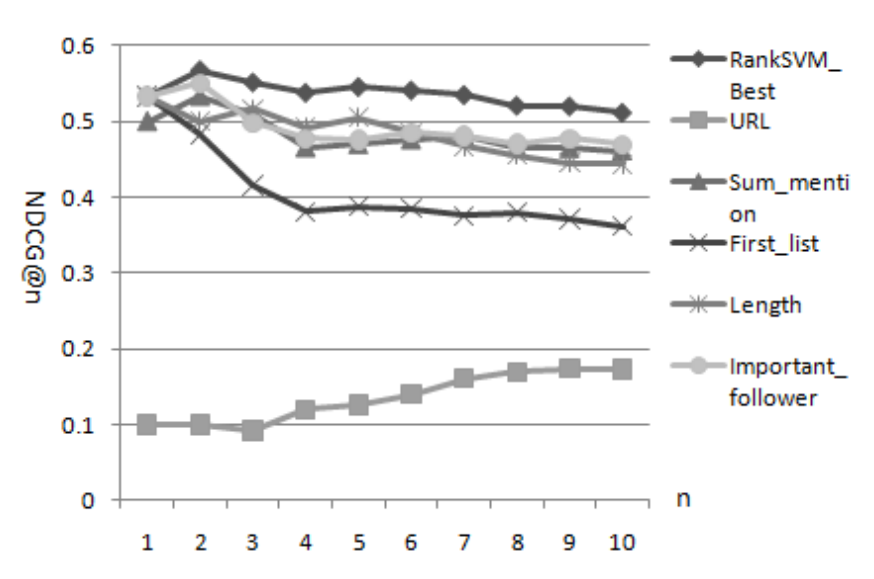
\epsfig{file=img/p2_results_features.png, width=0.45\textwidth}
\caption{Importance of Each Feature}
\end{figure}

% =========================
% =========================
% =========================

%\section{Related Work}

% =========================
% =========================
% =========================

\section{Conclusion}



\bibliographystyle{abbrv}
\bibliography{bibliography}  

\balancecolumns

\end{document}
